\documentclass[11pt,a4paper]{article}

% ---------- Encoding, fonts, micro-typography ----------
\usepackage[T1]{fontenc}
\usepackage[utf8]{inputenc}
\usepackage{lmodern}
\usepackage[final]{microtype}

% ---------- Page geometry ----------
\usepackage[a4paper,margin=1in]{geometry}
\usepackage{setspace}
\onehalfspacing

% ---------- Math ----------
\usepackage{mathtools, amssymb, amsthm}
\numberwithin{equation}{section}

% ---------- Lists, tables ----------
\usepackage{enumitem}
\usepackage{booktabs}
\usepackage{array}

% ---------- Graphics & colors ----------
\usepackage{graphicx}
\usepackage[dvipsnames]{xcolor}

% ---------- TikZ (figures) ----------
\usepackage{tikz}
\usetikzlibrary{arrows.meta,calc,positioning,fit,shapes.symbols,patterns}

% ---------- Unicode safety (common symbols) ----------
\usepackage{newunicodechar}
\newunicodechar{→}{$\to$}
\newunicodechar{←}{$\leftarrow$}
\newunicodechar{↔}{$\leftrightarrow$}
\newunicodechar{≥}{$\ge$}
\newunicodechar{≤}{$\le$}
\newunicodechar{—}{---}

% ---------- Hyperref ----------
\usepackage[unicode=true,colorlinks=true,linkcolor=MidnightBlue,citecolor=ForestGreen,urlcolor=RoyalBlue,psdextra]{hyperref}
\hypersetup{
  pdftitle={Normalized, Verifiable Computation: A Proposal},
  pdfauthor={},
  pdfsubject={},
  pdfkeywords={}
}

% ---------- Theorem styles (optional) ----------
\theoremstyle{plain}
\newtheorem{theorem}{Theorem}[section]
\newtheorem{lemma}[theorem]{Lemma}
\theoremstyle{definition}
\newtheorem{definition}[theorem]{Definition}
\theoremstyle{remark}
\newtheorem{remark}[theorem]{Remark}

% =====================================================
% Figure 2 (Gauge) — styles + one safe configuration macro
% =====================================================

% Visual palette (neutral)
\definecolor{ClampGreen}{RGB}{51,153,102}
\definecolor{ClampAmber}{RGB}{226,169,0}
\definecolor{ClampRed}{RGB}{204,68,68}
\definecolor{ClampGray}{gray}{0.35}

\tikzset{
  clamp/arc/.style={line cap=round, line join=round},
  clamp/tick/.style={ClampGray, line width=0.6pt},
  clamp/label/.style={ClampGray, font=\small},
  clamp/title/.style={ClampGray, font=\bfseries\footnotesize},
  clamp/metric/.style={ClampGray, font=\sffamily\scriptsize},
  clamp/dot/.style={fill=ClampGray, draw=white, line width=0.4pt}
}

% A single source of truth for the gauge geometry.
% Args:
%  #1 = outer radius (e.g., 3.2cm)
%  #2 = inner radius (e.g., 2.2cm)
%  #3 = start angle (deg, left end; e.g., 210)
%  #4 = end angle   (deg, right end; e.g.,  -30)
%  #5 = green fraction   in [0,1] of the total sweep (e.g., 0.50)
%  #6 = amber fraction   in [0,1] of the total sweep (e.g., 0.35)
%  #7 = pointer fraction in [0,1] position along sweep (e.g., 0.62)
\newcommand{\ClampConfig}[7]{%
  % store as lengths/dimens inside a TikZ pic
  \tikzset{
    declare function={
      clampStart   = #3;
      clampEnd     = #4;
      clampSpan    = (clampEnd - clampStart);
      fracGreen    = #5;
      fracAmber    = #6;
      fracRed      = max(0,1 - fracGreen - fracAmber);
      % guard: clamp fractions
      gEnd         = clampStart + clampSpan*fracGreen;
      aEnd         = gEnd       + clampSpan*fracAmber;
      pointerAng   = clampStart + clampSpan*#7;
    }
  }
  \def\ClampOuter{#1}%
  \def\ClampInner{#2}%
}

% Draw command (uses the parameters populated by \ClampConfig)
\newcommand{\DrawClamp}{%
  \begin{tikzpicture}[x=1pt,y=1pt]
    % Convert radii to pt for calc
    \pgfmathsetmacro{\rOuter}{\ClampOuter/1pt}
    \pgfmathsetmacro{\rInner}{\ClampInner/1pt}

    % Background ring (light gray guide)
    \path[draw=ClampGray!20,line width=8pt,clamp/arc]
      (0,0) ++(clampStart:\rOuter) arc [start angle=clampStart, end angle=clampEnd, radius=\rOuter];

    % Three arcs: green, amber, red
    \path[draw=ClampGreen,line width=8pt,clamp/arc]
      (0,0) ++(clampStart:\rOuter) arc [start angle=clampStart, end angle=gEnd, radius=\rOuter];

    \path[draw=ClampAmber,line width=8pt,clamp/arc]
      (0,0) ++(gEnd:\rOuter) arc [start angle=gEnd, end angle=aEnd, radius=\rOuter];

    \path[draw=ClampRed,line width=8pt,clamp/arc]
      (0,0) ++(aEnd:\rOuter) arc [start angle=aEnd, end angle=clampEnd, radius=\rOuter];

    % Pointer (neutral)
    \draw[ClampGray, line width=1pt]
      (0,0) -- ++(pointerAng:\rOuter-6);

    % Pointer dot
    \fill[clamp/dot] (0,0) circle[radius=2.2pt];

    % Tick marks (5 ticks)
    \foreach \k in {0,...,5}{
      \pgfmathsetmacro{\tA}{clampStart + \k*(clampSpan/5)}
      \draw[clamp/tick]
        (0,0) ++(\tA:\rOuter+2) -- ++(\tA:6);
    }

    % Labels
    \node[clamp/title, anchor=south] at (0,\rOuter+18) {Composite Safety Envelope};
    \node[clamp/label, anchor=north west] at (gEnd:\rOuter+12) {stable};
    \node[clamp/label, anchor=north]     at (aEnd:\rOuter+16) {governed};
    \node[clamp/label, anchor=north east]at (clampEnd:\rOuter+12) {halt};

    % Legend metrics (example placeholders; replace as needed)
    \node[clamp/metric, anchor=north west] at (-0.72*\rOuter, -0.9*\rOuter)
      {$\text{FoS margin} \ge 0$};
    \node[clamp/metric, anchor=north west] at (-0.72*\rOuter, -0.9*\rOuter-14)
      {$\rho_{\text{STL}} \ge 0$};
    \node[clamp/metric, anchor=north west] at (-0.72*\rOuter, -0.9*\rOuter-28)
      {$\text{KKT/Conservation: PASS}$};
  \end{tikzpicture}%
}

\begin{document}
\maketitle

\begin{abstract}
\noindent
We propose a research--neutral, safety--first program for verifiable computation.
Every consequential step emits a typed \receipt{} with deterministic encodings; header--only aggregation
produces a proof surface (a Merkle root) that auditors can check from bytes. Norms are specified in temporal logic and gated in CI via \smt; control is formulated as distributionally robust optimization (\dro) with level--1 optimality and conservation receipts and level--2 stability via cached \pr/\iss{} certificates with revocation. We formalize the evidence algebra, selective disclosure, mechanized governance (monotone safety), and operational obligations. The result is a practical path from assumed trust to provable trust.
\end{abstract}

\section{Objectives and Scope}
\label{sec:objectives}
Our objectives are domain--agnostic:
\begin{enumerate}[label=\textbf{O\arabic*.}]
  \item \textbf{Compositional evidence.} Receipts compose over time and parallelism.
  \item \textbf{Determinism by design.} Canonical encodings; pinned environments; replayable transcripts.
  \item \textbf{Mechanized governance.} Norms are machine--checkable and monotone under revision.
  \item \textbf{Transparent control.} Distributed uncertainty, robust objectives, explicit certificates.
  \item \textbf{Selective disclosure.} Privacy via payload commitments and field--level proofs.
\end{enumerate}

\section{Acceptance Coordinates and Unknowns}
\label{sec:acceptance}
Let $Q=\prod_{i=1}^d Q_i$ be acceptance coordinates with preorder $\preceq$. Partition axes into $M$ (``max'' channels) and $S$ (``sum'' channels) and define coordinatewise
\[
(x \sqcap y)_i :=
\begin{cases}
\max(x_i,y_i), & i\in M,\\[3pt]
x_i+y_i, & i\in S.
\end{cases}
\]
Each $Q_i$ contains an absorber $\top^{(i)}_{\text{unk}}$ that isolates unknowns to axis $i$.
Adapters $g$ are monotone homomorphisms with $g(\varnothing)=\top_{\text{unk}}$ and preserve $\sqcap$.
This yields a sound calculus for uncertainty (intervals, sub--Gaussian envelopes, Wasserstein balls) while prioritizing monotonic propagation.

\section{Receipts, Proof Surface, and Selective Disclosure}
\label{sec:receipts}
A \receipt{} splits into a canonical \emph{header} (schema id, predicate id, verdict, \code{prev\_digest}, \code{payload\_root}, \code{envlock\_digest}, hash suite) and a \emph{payload} committed by a Merkle root. The \emph{proof surface} is a Merkle root over canonical headers only; it detects header tampering and supports redaction: payload fields are revealed with inclusion proofs against \code{payload\_root} while the surface remains invariant.

\begin{figure}[h]
  \centering
  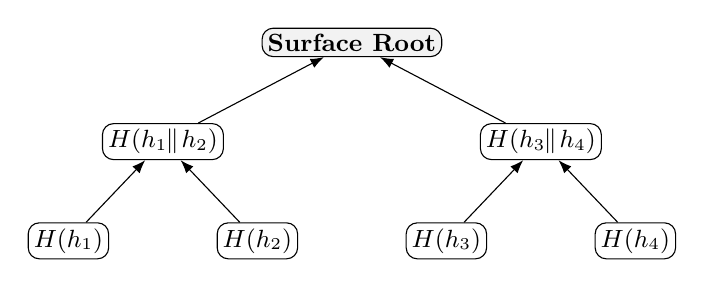
\begin{tikzpicture}[x=1.2cm,y=0.9cm,>=Latex]
    % leaves
    \node (l1) at (0,0) [draw,rounded corners,inner sep=2pt]{\small $H(h_1)$};
    \node (l2) at (2,0) [draw,rounded corners,inner sep=2pt]{\small $H(h_2)$};
    \node (l3) at (4,0) [draw,rounded corners,inner sep=2pt]{\small $H(h_3)$};
    \node (l4) at (6,0) [draw,rounded corners,inner sep=2pt]{\small $H(h_4)$};
    % level 1
    \node (a) at (1,1.4) [draw,rounded corners,inner sep=2pt]{\small $H(h_1\!\!\parallel\! h_2)$};
    \node (b) at (5,1.4) [draw,rounded corners,inner sep=2pt]{\small $H(h_3\!\!\parallel\! h_4)$};
    % root
    \node (r) at (3,2.8) [draw,rounded corners,inner sep=2pt,fill=gray!10]{\small \textbf{Surface Root}};
    % edges
    \draw[->] (l1) -- (a);
    \draw[->] (l2) -- (a);
    \draw[->] (l3) -- (b);
    \draw[->] (l4) -- (b);
    \draw[->] (a) -- (r);
    \draw[->] (b) -- (r);
  \end{tikzpicture}
  \caption{Proof surface: Merkle root over canonical \textit{headers} (not payloads).}
  \label{fig:surface}
\end{figure}

\paragraph{Audit hook.}
Any single--byte mutation in a header flips the surface root with overwhelming probability (collision resistance of $H$). Payload redaction leaves the root unchanged; inclusion proofs verify revealed fields against \code{payload\_root}.

\section{Norms: STL with SMT Gating}
\label{sec:norms}
Norms are stated in Signal Temporal Logic (\stl) with quantitative semantics; bounded monitors compile to \smt--LIB (QF\_LRA) and gate changes in CI. Dense--time properties are monitored via robust--satisfaction intervals; the lower bound is enforced online for soundness under discretization.

\section{Control as DRO with Receipts}
\label{sec:dro}
Control is posed as a distributionally robust program over a Wasserstein ball $\mathcal{B}_\varepsilon^p(P_0)$. Runtime artifacts:
\begin{itemize}
  \item \textbf{Level--1 receipts:} convex class declaration (QP/SOCP/SDP), \kkt{} residuals and duality gap within tolerances; conservation receipts verifying $\Delta V$ vs.\ declared spend.
  \item \textbf{Level--2 certificates:} \pr/\iss{} from an audited cache keyed by component digests; revocation checked before use.
\end{itemize}

\section{Mechanized Governance (Monotone Safety)}
\label{sec:governance}
Let $MF(N)$ be must--fail IDs in norms bundle $N$. CI enforces $MF(N_t)\subseteq MF(N_{t+1})$.
Optionally, \smt{} proves entailment between \stl{} revisions. Batches are summarized by epoch receipts committing prior headers so archival does not break verification.

\section{Rails and Clamp States}
\label{sec:rails}
Rails define banded operating regions (Green/Amber/Red) with hysteresis and dwell; transitions are driven by guard margins and certificate status. Policies emit selective--disclosure receipts and can gate pipeline modes.

\begin{figure}[t]
  \centering
  % Configure once for this figure instance:
  % \ClampConfig{outer radius}{inner radius}{start angle}{end angle}{green frac}{amber frac}{pointer frac}
  \ClampConfig{3.2cm}{2.1cm}{210}{-30}{0.50}{0.35}{0.62}
  \DrawClamp
  \caption{Composite safety envelope (illustrative). The pointer indicates a
  normalized state estimate within a three-band envelope (stable/governed/halt).
  Bands and pointer are driven by formal metrics (e.g., STL robustness, Factor-of-Safety,
  and certificate verdicts); receipts make these quantities auditable without revealing
  sensitive payloads.}
  \label{fig:composite-envelope}
\end{figure}

\section{Short Proofs}
\label{sec:proofs}
\begin{proposition}[Header Tamper Detectability]
If $H$ is collision--resistant and the surface root is a Merkle root over canonical headers, any header byte mutation changes the root with overwhelming probability.
\end{proposition}
\begin{proof}
A changed header yields a different leaf hash; Merkle recomputation propagates to the root unless a collision occurs in $H$.
\end{proof}

\begin{lemma}[Redaction Invariance]
If a header commits to payload root $\rho$, selective disclosure that preserves $\rho$ leaves the surface root unchanged.
\end{lemma}
\begin{proof}
The surface aggregates headers only; inclusion proofs check revealed fields against $\rho$.
\end{proof}

\begin{proposition}[Distributivity of Evidence Aggregation]
Let $A,B$ be sets of valid chains; let $c$ be a valid chain. Then
$c\ast (A\sqcup B)=(c\ast A)\sqcup (c\ast B)$.
\end{proposition}
\begin{proof}
Prefixing by $c$ maps each chain to a longer chain and distributes over set union pointwise.
Canonical sorting of header bytes makes aggregation order--insensitive.
\end{proof}

\begin{proposition}[Monotone Safety]
If CI enforces $MF(N_t)\subseteq MF(N_{t+1})$ for all $t$, safety obligations are monotone nondecreasing.
\end{proposition}
\begin{proof}
Set inclusion prevents removal of any previously required must--fail; additions tighten obligations; equality preserves them.
\end{proof}

\section{Threats and Mitigations}
\label{sec:threats}
\begin{center}
\renewcommand{\arraystretch}{1.1}
\begin{tabular}{@{}p{0.28\linewidth}p{0.66\linewidth}@{}}
\toprule
\textbf{Threat} & \textbf{Mechanized Mitigation}\\
\midrule
Supply--chain drift & EnvLock by digest; deterministic encodings; receipts bind \code{envlock\_digest}.\\
Ledger tampering & Header--only surface (Merkle root); any header byte flip changes root.\\
Signature malleability & Normative \cose{} over deterministic \cbor{}; Ed25519 (\code{alg=-7}).\\
DoS via growth & Deterministic batching; epoch summaries; archival with root verification.\\
Privacy leakage & Selective disclosure with payload proofs; headers suffice for chain checks.\\
Controller instability & L1 receipts (\kkt, Conservation); L2 \pr/\iss{} from revocation--checked cache.\\
\bottomrule
\end{tabular}
\end{center}

\section{Verification Obligations}
\label{sec:obligations}
\begin{itemize}
  \item \vo-ROOT-EQUAL: identical inputs $\Rightarrow$ identical surface roots across platforms.
  \item \vo-LEDGER-TAMPER: single--byte header mutations alter the root.
  \item \vo-SD-CORRECT: selective--disclosure proofs verify against \code{payload\_root}; root unchanged.
  \item \vo-NB-MONO: $MF(N_t)\subseteq MF(N_{t+1})$ in CI; deltas receipted.
  \item \vo-KKT-RESID: convex class declared; residuals and dual gap $\le$ tolerances.
  \item \vo-CONS-BAL: conservation: observed $\Delta V$ matches declared spend (within tolerance).
  \item \vo-PR/ISS-CACHE: L2 certificates only accepted from non--revoked cache entries.
\end{itemize}

\section{Operational Checklists}
\label{sec:checklists}
\paragraph{Proof Surface (header--only).}
Input: headers $H=\{h_1,\dots,h_n\}$ (canonical bytes)
\begin{enumerate}[nosep]
  \item Sort $H$ lexicographically (byte--wise).
  \item Compute leaves $L_i=H(h_i)$.
  \item Build binary Merkle tree over $\{L_i\}$.
  \item Output root $R$.
\end{enumerate}

\paragraph{Selective Disclosure Verification.}
Input: header $h$ (with \code{payload\_root} $\rho$), revealed fields and inclusion proofs. Verify each Merkle path to $\rho$; if all paths verify, accept fields as authentic w.r.t.\ $\rho$.

\paragraph{Level--1 \dro/\kkt{} Receipt.}
Input: transcript $T$, convex class $C$, residuals $(r_{\text{stat}},r_{\text{pri}},r_{\text{dual}})$, duality gap $g$, tolerances $\tau$. Require $C\in\{\text{QP},\text{SOCP},\text{SDP}\}$ and all residuals/gap $\le \tau$.

\section{Assumptions and Limitations}
\label{sec:limits}
Collision resistance reduces to assumptions on $H$ and EdDSA; determinism requires a fixed toolchain and canonical encodings (cross--ISA floating point may need fixed--point or constrained kernels). Dense--time \stl{} monitoring uses robust intervals (sound but conservative).
L2 certificate acceptance is via audited cache with revocation; full online recomputation is out of scope for high--rate loops.

\section{Context and Prior Art (Neutral)}
\label{sec:context}
This program synthesizes reproducible supply--chain attestations (deterministic builds; byte--identical artifacts), transparent logs with tamper--evident commitments (hash--chained receipts; Merkle proof surfaces), and formal control/verification for runtime safety (\stl/\smt{} gating; CLF/CBF; \kkt/\pr/\iss{} receipts). The contribution is a normalized architecture in which every consequential step emits a typed, auditable, selectively disclosable \receipt{}, enabling independent conformance checks and reproducible evaluation.

\section{Conclusion}
\label{sec:conclusion}
We present a neutral, safety--first architecture for verifiable computation with compositional receipts, deterministic encodings, formal norms and governance, \dro{} control with explicit certificates, and privacy by selective disclosure. Short proofs, obligations, and checklists make the program practically auditable.

\paragraph{Compilation Notes.}
No math in section titles; Unicode punctuation mapped; no bold small caps. If you see an \emph{Overfull \texttt{\string\hbox}} in long URLs, wrap them with \verb|\url{...}|.

\end{document}
